\documentclass{article}
\usepackage[utf8]{inputenc}
\usepackage[polish]{babel}
\usepackage{polski}
\usepackage{enumerate}
\usepackage{natbib}
\usepackage{graphicx}
\usepackage{geometry}
\usepackage{float}

\newgeometry{tmargin=2.3cm, bmargin=2.5cm, lmargin=2.5cm, rmargin=2.5cm}

\makeatletter
\newcommand{\linia}{\rule{\linewidth}{0.4mm}}
\renewcommand{\maketitle}{\begin{titlepage}
    \vspace*{1cm}
    \begin{center}
    Politechnika Wrocławska\\
    AiR ARR\\
 Projekt zespołowy
    \end{center}
      \vspace{3cm}
    \begin{center}

     \LARGE \textsc {\@title}
         \end{center}
     \vspace{1cm}

    \begin{center}
    \textit{ Autorzy:}\\
   \textit{\@author}
     \end{center}
      \vspace{1cm}

     \begin{center}

    Prowadzący:
  dr inż. Krzysztof Arent
    \end{center}

    \vspace*{\stretch{6}}
    \begin{center}
    \@date
    \end{center}
  \end{titlepage}
}
\makeatother
\author{Beata Berajter\\
Dawid Brząkała\\
Dorota Gidel\\
Katarzyna Wądrzyk\\
Ada Weiss\\
Małgorzata Witka-Jeżewska\\
 }
\title{SensGlove\\Raport z przebiegu projektu}

\begin{document}

\maketitle
\newpage
\tableofcontents
\newpage



\section{Kryteria ewaluacji}
Komponenty powinny działać każde z osobna oraz współdziałać jako kompletne stanowisko do pobierania sygnałów i biosygnałów. Użytkownik powinien mieć możliwość wykonywania ruchów w obrębie przynajmniej jednego metra od stanowiska. Rękawiczka pomiarowa powinna mieć umieszczone czujniki w taki sposób, aby nie ograniczała ruchów ani tym bardziej nie krępowała ich. Pomiary przesyłane mają być w czasie rzeczywistym, a ich podgląd zapewnić ma program wizualizujący je.
\begin{enumerate}
	\item Założenie rękawiczki.
	\item Poruszanie palcami.
	\item Obserowanie przebiegów pomiarów.
	\item Rozpoczęcie pomiaru.
	\item Zapis pomiaru.
	\item Sprawdzenie katalogu, w którym dokonano zapisu.
\end{enumerate}
%%%%%%%%%%%%%%%%%%%%%%%%%
% Ogólnie:
% zrealizowane części projektu
% sposób ich zrealizowania
% niezrealizowane
% dlaczego nie
%
%
%
% Pozmieniałam tytuły dla punktu 2.1, prosze zrobić coś w tym właśnie stylu, chyba że macie lepsze propozycje - można tak jak w punkcie 2.4 robić
%
%
% UWAGA! Tekst specyfkacji zostawiam po to, zebyscie nei musieli szukać! Należy go usunać albo chociaż zmienić na swoje potrzeby
%%%%%%%%%%%%%%%%%%%%%%%%%
\section{Przebieg prac dla poszczególnych komponentów}
\subsection{Rękawiczka sensoryczna}
Osoby przydzielone do zadania: Dorota Gidel, Katarzyna Wądrzyk.
\subsubsection{Spełnione wymagania użytkownika}
%np. na rękawiczce zostało przymocowanych tyle a tyle sensorów poprzez rpzyklejenie ich do rękawiczki i przyszycie + kapturki

\subsubsection{Spełnione funkcjonalności}
%została zakupiona rękawiczka itd., dlaczego inny rozmiar

\subsubsection{Kryteria ewaluacji}
% np. w tym momencie rękawiczka spełnai następujace kryteria:


\subsection{Interfejs sprzętowy}

Osoby przydzielone do zadania: Beata Berajter i Dawid Brząkała. \\


%odniesc sie trzeba jakos do tych kryteriów, co juz jest zrobione, moze zdjecie pcb, 
\subsection{Schemat płytki pcb i wyprowadzenie pinów układu}

\begin{figure}[h!]
    \centering
    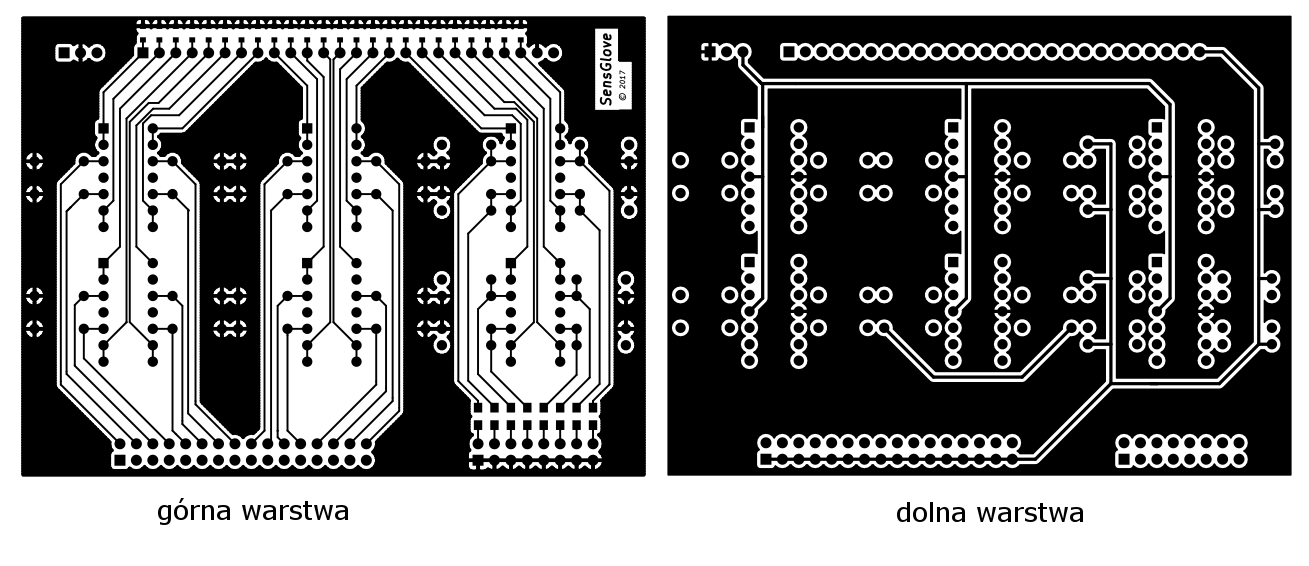
\includegraphics[scale=0.6]{pcb.png}
    \caption{Schemat płytki pcb}
    \label{rys:pcb}
\end{figure}

\begin{figure}[h!]
    \centering
    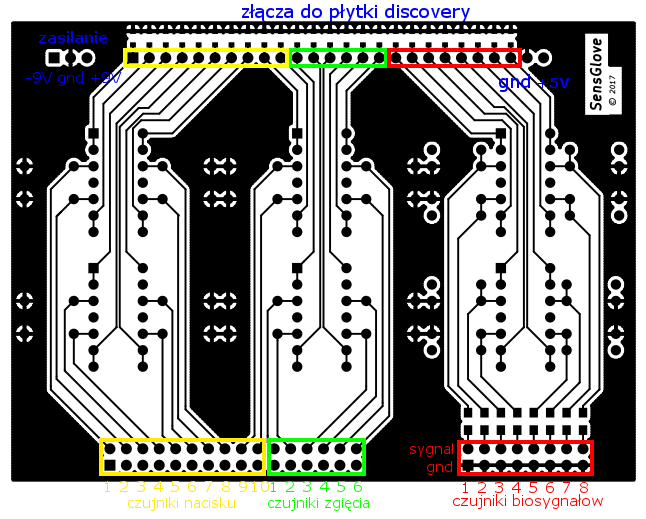
\includegraphics[scale=0.6]{pinout.png}
    \caption{Wyprowadzenie pinów płytki pcb}
    \label{rys:pinout}
\end{figure}

\subsubsection{Kryteria ewaluacji}
Poprawność odczytu sygnałów przez układ wzmacniaczy sygnałów sprawdzono poprzez podłączenie potencjometrów w miejsce czujników i pomiar napięć na wyjściu. Sprawdzono również współpracę z rękawiczką. 
Następnym etapem będzie podłączenie układu do płytki Discovery i przesył uzyskanych wyników do komputera. 
Poprawność samej transmisji sprawdzona zostanie poprzez wysyłanie zaprogramowanych wcześniej przykładowych wiadomości i odczytywanie ich w komputerze poprzez program do monitowania portów COM.

\begin{enumerate}
	\item Wgranie na płytkę Discovery programu przesyłającego symulowanych danych z płytki do komputera użytkownika.
	\item Sprawdzenie miernikiem lutów i ścieżek na układzie ze wzmacniaczami.
	\item Podłączenie potencjometrów symulujacych czujniki do płytki Dicovery w celu sprawdzenia poprawności działania przetworników ADC.
	\item Podłącznie wzmacniaczy do płytki Dicovery i powtórzenie testu z użyciem potencjometrów.
\end{enumerate}


%%%%%%%%%%%%%%%%%%%%%%%%%
\subsection{Program do akwizycji danych}

Osoby przedzielone do zadania: Ada Weiss, Małgorzata Witka-Jeżewska
\subsection{Opis klas programu}
Dokładny opis klas i poszczególnych parametrów tworzony jest za pomocą programu Doxygen.
\begin{figure}[h!]
    \centering
    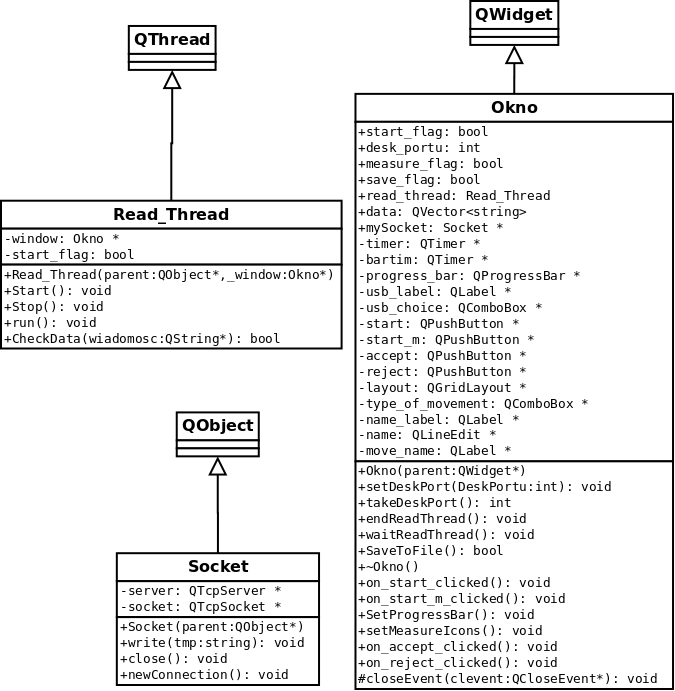
\includegraphics[scale=0.4]{autodia.png}
    \caption{Diagram klas programu}
    \label{rys:autodia}
\end{figure}

\begin{figure}[h!]
    \centering
    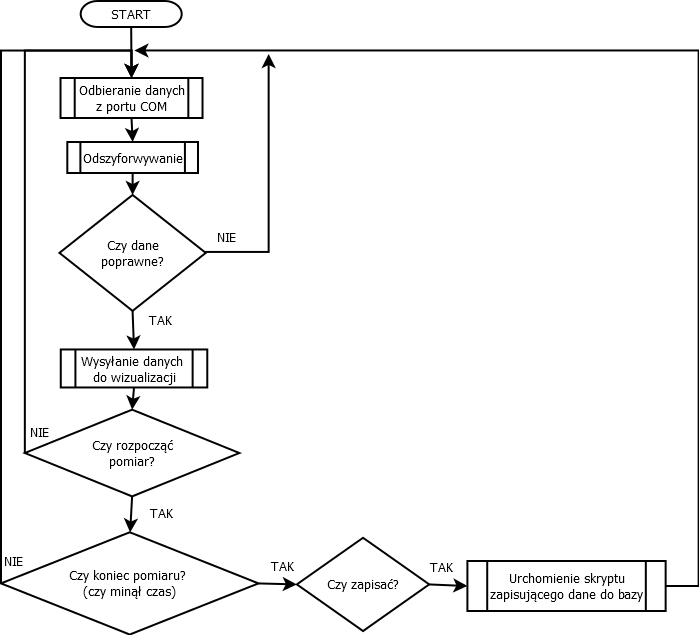
\includegraphics[scale=0.6]{programdia.png}
    \caption{Schemat ideowy działania programu}
    \label{rys:programdia}
\end{figure}

\subsection{Opis działania programu}

Interfejs graficzny programu został napisany z wykorzystaniem klas biblioteki Qt5 i został zaprezentowany na rys. \ref{rys:okno}. 
\begin{figure}[h!]
    \centering
    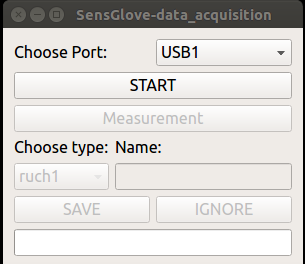
\includegraphics[scale=0.6]{okno.png}
    \caption{Okno główne programu}
    \label{rys:okno}
\end{figure}

Zasada działania została przedstawiona na rys. \ref{rys:programdia}. 
Pierwszym krokiem jest wybór portu USB i wciśnięcie przycisku start, co uruchamia konfiguracje wybranego portu USB. W przypadku braku podłączonego urządzenia na danym porcie wyświetlany jest komunikat przedstawiony na rys. \ref{rys:oknousb}. Kliknięcie "Yes" umożliwia ponowny wybór, a "No" kończy pracę programu.\\
\begin{figure}[h!]
    \begin{center}
    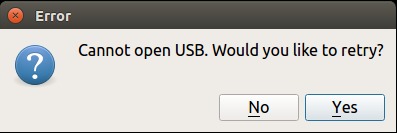
\includegraphics[scale=0.6]{oknousb.png}
    \caption{Komunikat o błędnym otwarciu USB.}
    \label{rys:oknousb}
    \end{center}
\end{figure}
Dane są odczytywane z poru USB w oddzielnym wątku Read\_thread, dziedziczącego po QThread. Zapewnia to odpowiednio szybką pracę programu. W tym samym wątku sprawdzana jest poprawność otrzymanej wiadomości (obliczanie sumy kontrolnej, sprawdzanie dlugości ciągu znaków) oraz wysyłanie danych do Socketu, który również został zaprogramowany z wykorzystaniem bibliotek Qt5 (klasa Socket).

W przypadku aktywowania przycisku "Measurment" aktywowany jest timer (na 2s) i dane te są zapisywane w wektorze 2000x23, z którego to jest możliwość zapisu danych do pliku w przypadku akceptacji pomiaru po jego ukończeniu. Widok okna w trakcie pomiaru przedstawia \rys{rys:oknopomiar}.
\begin{figure}[h!]
    \centering
    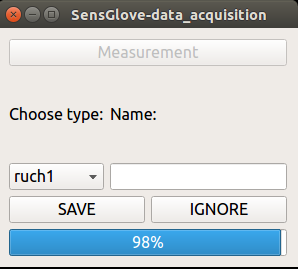
\includegraphics[scale=0.6]{oknopomiar.png}
    \caption{Okno główne programu w trakcie pomiaru}
    \label{rys:oknopomiar}
\end{figure}

Akceptacja pomiaru wymaga również podania imienia użytkownika oraz wyboru ruchu który jest wykonywany. Program wywołuje po zapisie do pliku skrypt który umieszcza plik w bazie danych.

Można również dany pomiar zignorować, np. w przypadku stwierdzenia, że został on błędnie wykonany.

\subsubsection{Format danych}
Ramka danych:
\begin{itemize}
    \item znak X,
    \item 23 sygnały z czujników w postaci 4 znaków w systemie szesnastkowym,
    \item suma kontrolna w postaci dwóch znaków w systemie szesnastkowym,
    \item znak końca linii \backslash r \backslash n;
\end{itemize}

\subsubsection{Raport z ewaluacji}
Do symulowania danych wejściowych zaprogramowano płytkę STM32F476G Discovery tak, aby nadawała przykładowe dane w ustalonym przez nas formacie poprzez odpowiednią konfigurację USB. \\
Do sprawdzenia poprawności przesyłu danych wykorzystany został program telnet. Dane nadawane są na porcie 2666 (planowane jest dodanie możliwości wyboru portu, na którym dane będą nadawane). Przesył danych był poprawny. \\
Dane były również wysyłane do programu do wizualizacji rękawiczki poprzez wspólny router Wi-Fi do drugiego komputera. Przesyłanie odbywało się bez zarzutów.

%%%%%%%%%%%%%%%%%%%%%%%%%
\subsection{Baza danych}
Osoby przydzielone do zadania: Beata Berajter, Dorota Gidel.
\subsubsection{Wymagania użytkownika}

\subsubsection{Funkcjonalność}

%trzeba odniesc sie do tych kryteriów, czy to działa tak jak miało itd.. dlatego są zostawione potem trzeba je usunąć, tutaj troszke zmieniła sie koncepcja (cos z tą data prawda? ) czy wgl będziemy robic to wyszukiwanie? 
\subsubsection{Kryteria ewaluacji}
Do sprawdzenie poprawności działania bazy danych zostanie wywołana funkcja obsługi bazy z przykładowymi argumentami i danymi z czujników. Zarówno wejściowym jak i wyjściowym efektem są pliki tekstowe. Zostaną utworzone przykładowe testowe pliki, dzięki którym będzie można porównać oraz sprawdzić poprawność przetworzonych danych.

\begin{enumerate}
	\item Wywołanie funkcji zapisu z przykładowymi danymi wejściowymi.
	\item Sprawdzenie katalogów z zapisanymi informacjami.
	\item Wywołanie funkcji znajdującej pomiary po osobie go wykonującej.
	\item Sprawdzenie odczytanych pomiarów.
\end{enumerate}


%%%%%%%%%%%%%%%%%%%%%%%%%
\subsection{Wizualizacja danych}
Osoby przydzielone do zadania: Dorota Gidel, Katarzyna Wądrzyk.
%rzeba odniesc sie do tych kryteriów, czy to działa tak jak miało itd.. dlatego są zostawione potem trzeba je usunąć
\subsubsection{Kryteria ewaluacji}
Działanie programu sprawdzone będzie pod kątem odbierania sygnału z rękawiczki oraz poprawnego wyświetlania danych na modelu 3D. \\
Gdy wysłany zostanie sygnał maksymalnego nacisku z czujnika na palcu wskazującym program go odczyta oraz wyświetli kolor czerwony na wizualizacji. Gdy zgięty zostanie dany palec u ręki, palec na modelu w programie również zostanie zgięty. Gdy kąty zgięcia oraz kolory nacisku będą się zgadzać, znaczyć to będzie, że aplikacja działa poprawnie. Dane te mogą być sztucznie symulowane i wysyłane do programu, by istniała możliwość testowania bez istnienia poprawnie działających komponentów systemu.

\begin{enumerate}
	\item Przesłanie  symulowanych danych z czujników do progamu.
	\item Sprawdzenie, czy wizualizacja pokrywa się z przewidywanym ruchem.
\end{enumerate}


\end{document}
